\documentclass[prb,11pt]{revtex4-1}

% preamble:

\usepackage{amsmath}    % need for subequations
\usepackage{graphicx}   % need for figures
\usepackage{verbatim}   % useful for program listings
\usepackage{color}      % use if color is used in text
\usepackage{subfigure}  % use for side-by-side figures
\usepackage{hyperref}   % use for hypertext links, including those to external documents and URLs
\raggedbottom           % don't add extra vertical space
\begin{comment}
\pagestyle{empty}       % use if page numbers not wanted
\end{comment}

\begin{document}

\title{Effective viscosity of polymer networks in the presence of cross-link slip}
\author{William McFadden}
\affiliation{University of Chicago, Biophysical Sciences Program, Chicago, IL 60615}

\date{1 January 2014}

\begin{abstract}
We are trying to describe the problem of what happens when cross-links relax stress in semi-flexible filament networks.  We have addressed the problem using a simplified model in which cross-links are allowed to slip past one another in a friction-like manner.  This model gives a prediction for the long timescale effective viscosity of the medium.  We have verified our solution using computational models of filaments in the limit where persistence length is much longer than filament length.  In this model, we find that network architectures and slip rates give rise to different modes of connectivity.
\end{abstract}

\maketitle

\section{Introduction}





Chemists have made synthetic systems that exhibit so called slide-ring cross-linking, but thus far this exact mechanism has not been seen in biological systems.  However, (some garbage experiments from biophysical journal that I know must exist because people put bullshit in biophysical journal all the time) have shown that multivalent crosslinks can effectively slide under a load.

\section{The Model}
Here I will include math and equations that explain what it is that I am talking about when I talk about a model.  It will involve writing the semi-flexible filament potential and then writing the coupling equation.  These are just placeholders for now, while I write these things out by hand first.

Introduce wormlike chain model
In the worm-like chain model, semi-flexible polymers are modeled as continuous curves s(x), 
\begin{equation}
{\cal H} =\frac{1}{2}\kappa \int ds(\nabla^2\mathbf{u})^2 + \frac{1}{2}\mu \int ds \left ( \frac{dl(s) }{ds} \right )^2
\end{equation}

Introduce the formation of isotropic networks of wormlike chains.

Introduce connection points as friction points
{In previous work, crosslinks have been taking to be either perfectly rigid attachment points (HLM) or extended springlike structures (Taeyoon).  In addition, any mechanism of detachment is either absent (HLM) or governed by full detachment and full reattachment events(other).  In our model, we aim to create a more simple picture of crosslink stress relaxation based on .}

Appendix material on connecting crosslink unbinding and corsslink slip

Introduce form of coupling equation between 

\begin{equation}
\mathbf{F_{friction}} = \delta \zeta \cdot \int ds \: (\mathbf{v(s)}-\mathbf{v_0(s)}) \: p(s)
\end{equation}

\section{Analytical Results}
And this is where I prove by hand that some great amazing things can be seen about the system if we just take our little averages the right way.

\begin{equation}
\mathbf{\sigma} = \frac{1}{D}\sum_{filaments}\: \sum_{crosslinks}\delta \zeta \cdot (\mathbf{v_i}-\mathbf{v_0})\end{equation}

\begin{equation}
\mathbf{\sigma} =  \frac{1}{D}\sum_{filaments}\:  \delta \zeta \cdot \int_0^L ds \: (\mathbf{v(s)}-\mathbf{v_0(s)}) \:\frac{1}{l_c} = \sum_{filaments}\:  \frac{\delta \zeta \dot \gamma L}{l_c} \cos \theta \cdot (x_l + \frac{L}{2} \cos \theta)
\end{equation}

\begin{equation}
\mathbf{\sigma} =  \frac{1}{D} \int_0^L dx_l \int_{-\arccos (\frac{x_l}{L})}^{\arccos (\frac{x_l}{L})}d\theta \frac{\delta \zeta \dot \gamma L}{l_c} \cdot \frac{h}{Ll_c}\cdot \frac{\pi}{2}\arccos(x_l/L) (x_l \cos \theta + \frac{L}{2} cos^2\theta)
\end{equation}

\begin{equation}
\mathbf{\sigma} = \frac{L^2}{l_c^2} \cdot \delta \zeta \cdot \frac{2}{\pi}(\pi(1+1/6)-20/9) \approx \frac{L^2}{l_c^2} \cdot \delta \zeta
\end{equation}

\begin{figure}[h!]
\centering
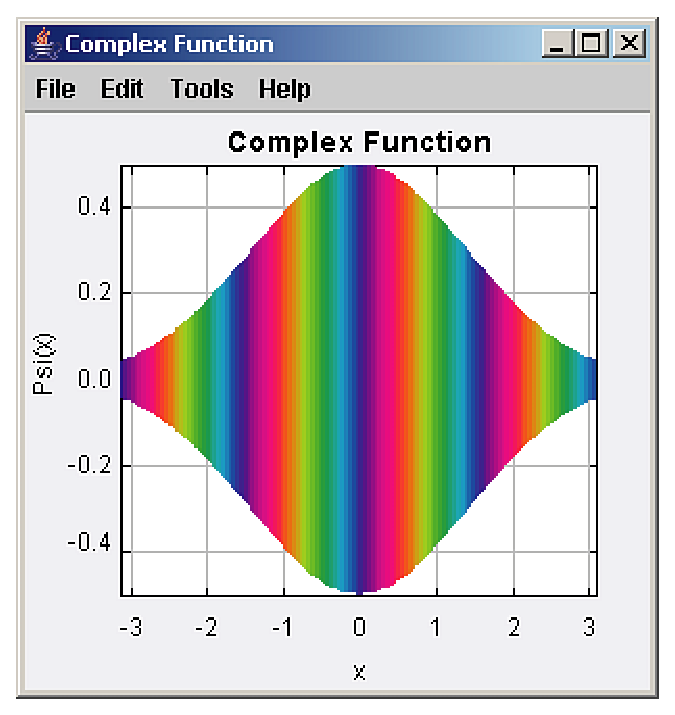
\includegraphics[scale=0.6]{phase}
\caption{\label{fig:phase}And here is your predicted phase diagram.}
\end{figure}


\section{Simulation Results}

And here, I show the simulation results, which fall into three categories, 1) the frequency falloff can be explained by heterogeneity in length, 2) the steady state effective viscosity matches the theoretical prediction in a range of parameter space, 3) the network tearing time drops as the effective viscosity drops to 0

We have implemented a solution to the discretized form of our model equations.  

\begin{figure}[h!]
\centering
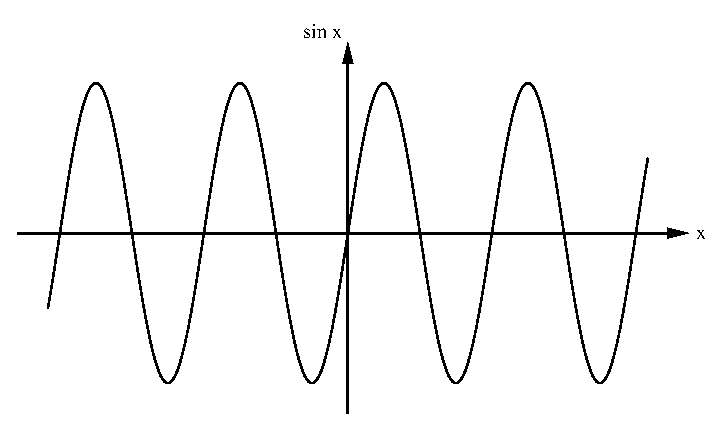
\includegraphics[scale=0.6]{sine}
\caption{\label{fig:sine}Show me a sine.}
\end{figure}

We can make figures bigger or smaller by scaling them. Figure~\ref{fig:sine}
has been scaled by 60\%.


\section{Simulation details}
And I think I'll probably include all the gory details of how my simulations work since I'll be wanting to have direct references to the code. 
\begin{verbatim}
double y0 = 10; // example of declaration and assignment statement
double v0 = 0;  // initial velocity
double t = 0;   // time
double dt = 0.01; // time step
double y = y0; // solved all problems
\end{verbatim}


\section{Discussion}

{\color{blue}{Finally I wax philosophical}},
{\color{green}{but}} {\color{cyan}{who is going pay for the ink?}}

\begin{thebibliography}{5}

\bibitem{latex}Helmut Kopka and Patrick W. Daly, \textsl{A Guide to
\LaTeX: Document Preparation for Beginners and Advanced Users} (Addison-Wesley, 2004), 4th ed.

\bibitem{website}Some useful links are
given at \url{<sip.clarku.edu/tutorials/TeX/>}.

\end{thebibliography}

\end{document}